\documentclass[11pt]{article}
\usepackage{amssymb}
\usepackage{graphicx}

\usepackage[outdir=./]{epstopdf}
\usepackage{etoolbox}
%\patchcmd{\maketitle}{\newpage}{}{}{}

%\DeclareGraphicsExtensions{.eps}

\usepackage{mathtools}
\usepackage{enumerate}
\usepackage{apacite}
\usepackage{listings}
\usepackage{multirow}
\usepackage{todonotes}
\usepackage{svg}
\usepackage{booktabs}
\usepackage{afterpage}
\usepackage[margin=1.25in]{geometry}

\newcommand{\den}[2][]{
\(
\left\llbracket\;\text{#2}\;\right\rrbracket^{#1}
\)
}


\newcommand{\KL}[2]{\ensuremath{D_{KL}({#1}\, \| \, {#2})}}
\newcommand{\E}[2]{\ensuremath{\mathbb{E}_{#1}\left [#2 \right]}}

\newenvironment{figurehere}
	{\def\@captype{figure}}
	{}

\setcounter{tocdepth}{2}
\usepackage{lipsum}
%\pagenumbering{gobble}
%\usepackage{apacite}

%\linespread{1}
\usepackage{textcomp}
\usepackage{lingmacros}
\usepackage{setspace}%\doublespacing 

\DeclareGraphicsRule{.tif}{png}{.png}{`convert #1 `dirname #1`/`basename #1 .tif`.png}
\graphicspath{{./figures/}}
 
%\makeatother

\title{Pr\'ecis of \\ \emph{Coordinating on Meaning in Communication} }
\author{Robert D. Hawkins \\ \small Department of Psychology, Stanford University}
\date{}

\begin{document}
%\thispagestyle{otherpage}

\maketitle

It is tempting to think of word meanings as entries in a dictionary shared by speakers of a language. 
Drop into any conversation between friends, however, and you wade into a stream of shorthand, jargon, slang, references, nicknames, and inside jokes --- some of which you may understand, but the rest of which may be meaningful to them alone. 
There is no guarantee, it seems, that any two speakers of a language will share the same dictionary.
To make matters worse, we live in an ever-changing world where we need to talk about new things.
There is also no guarantee that any dictionary could anticipate the meanings we will need to express in every new context.
If we cannot rely on the existence of a shared dictionary for coordination, then, what can we rely on?
How do we manage to understand one another so effortlessly in this patchwork landscape of meaning?

My dissertation investigates the cognitive mechanisms that allow individuals, and communities, to solve this challenge.
The core theoretical contribution of this work is an account of communication relaxing the assumption that speakers of a language share the same ``protocol.''
Instead, we propose that communication is better understood as a multi-agent meta-learning problem.
Agents must integrate background expectations about reliable community-wide conventions \cite{Lewis69_Convention} with new \emph{ad hoc}, partner-specific conventions constructed on the fly \cite{clark_using_1996,davidson_nice_1986}.
Chapters 1-2 formalize this proposal in a hierarchical Bayesian model and present simulation results capturing key effects from the literature. 
Chapter 3 evaluates an algorithm scaling this proposal to a recurrent neural network that interactively adapts to human partners.
Chapter 4 characterizes the dynamics of coordination in a large behavioral corpus of the classic Tangrams task. 
Chapter 5 tests how the communicative needs of the context shape the resulting \emph{ad hoc} conventions. 
Finally, Chapter 6 assesses the generality of the proposed mechanisms by examining coordination in a \emph{graphical} communication task. 

This work draws from , and developing computational cognitive models that give us mechanistic insight into how adaptive language use may be reverse-engineered from general principles of social cognition and learning. 
More broadly, this work opens avenues for future work to understand how social conventions are represented in the mind, how these conventions are shaped by our goals and environment, and how they give rise to the remarkable feats of social coordination that are so distinctive of human cultures \cite{hawkins2019emergence}.

\section*{Introduction}

Do people adapt at all? 
Representations v. decisions, i.e. updating cognitively deep latent meanings v. priming/alignment.

Under this view, knowledge of community-wide linguistic conventions supplies a useful but uncertain first guess about the linguistic meanings that will be shared with a new partner. 
Through interaction, these general expectations are gradually tuned to the local context via social inferences based on that partner's language use. 
As each party learns about the other and attempts to be understood under their updated model of partner-specific meaning, they coordinate on a system of meaning that is tailored to be efficient and accurate for their present purposes.
Finally, 

Computational models of meaning must explain both the speaker’s initial expectations about how words will be understood by novel partners and the dynamics of how these expectations may shift over the course of a particular conversation. In \ proposes a computational model that formalizes the problem of coordinating on meaning as hierarchical probabilistic inference, which I argue satisfies both of these conditions. Community- level expectations provide a stable prior, and dynamics within an interaction are driven by partner- specific learning.

Here we lay out the theoretical landscape and empirical evidence focusing on three key aspects of our theoretical approach: (1) the context-sensitive semantic priors that represent our initial uncertainty over what a novel partner is likely to mean by a word, (2) the path-dependence and increasing efficiency of our communicative behavior across even short periods of repeated interaction, and (3) the pattern of generalization from learning local interactions to new contexts and new partners. 

This review also provides scaffolding for the experimental paradigm used in Chapters 2 and 4 and introduces the phenomena that we capture with our simulations in Chapter 3.

The core of this work is an inferential model of convention formation that explains flexible and adaptive language use across extended interaction as a consequence of hierarchical probabilistic learning. Through observing their partner's usage, agents attempt to infer and adopt their partner's underlying lexicon using global conventions as a prior. When both agents independently adopt such a learning strategy, they align to one another, coordinating on and implicitly creating new, shared conventions. 


\vspace{1cm}

\section*{An inferential theory of convention formation}

In \textbf{Chapter 2}, we propose a hierarchical Bayesian model of convention formation that formalizes our proposal (see Fig. \ref{fig:modelschematic}): global conventions are learned and generalized over many extended interactions with many different people across a lifetime, and this shared semantic prototype is the backbone supporting rapid learning for new partners and situations. 

What cognitive mechanisms explain these phenomena? 
Recent probabilistic modeling framework which derives pragmatic considerations of language use from more generic computational principles of social cognition in rational agents.
%, specifically recursive probabilistic inference about the beliefs and intentions of rational agents. 
% \emph{Gricean pragmatics} due to their origins in Paul Grice's ``cooperative principle,'' operate within the production or comprehension of a single utterances. 
For example, listeners treat the literal meaning of a question as a cue to infer and address the underlying goal of the questioner {\color{Red} \textbf{\shortcite{hawkins_why_2015, hawkins_QA_2018}}}. 
And even though many labels may be literally true of an object, speakers refer to objects at an appropriate level of specificity given the other objects in context  {\color{Red} \textbf{\cite{graf_animal_2016, monroe2017colors}}}. 
They also increase the specificity of their utterances under additional uncertainty over what else might be in their partners' visual field {\color{Red} \textbf{\shortcite{hawkins_conversational_2016, hawkins2018speakers}}}.
While powerful, these models are unable to explain the flexibility and adaptiveness of conventions over time, as they are constructed on top of \emph{fixed} linguistic meanings.

A central aim of my dissertation work was to extend these models to capture how agents represent and rapidly coordinate on new conventions.% that explains the results of the above experiments. 
I have implemented this theory in a Bayesian model that relaxes the assumption of fixed word meanings in probabilistic pragmatics models and instead treats them as dynamic and learnable for different partners. 
This captures a functional view of linguistic conventions as solutions to coordination problems, in which every agent is simultaneously seeking to infer the conventions that other agents are using, in order to support successful communication. 
% assumes others are using some set of conventions and is trying to learn them such that they can be understood.  %: global conventions are learned and generalized over many extended interactions with many different people across a lifetime, and  this shared semantic prototype is the backbone supporting rapid learning for new partners and situations. 
This model successfully predicts coordination on idiosyncratic but path-dependent and stable form-meaning mappings in simulations, and shows that a preference for less costly utterances combined with learning gives rise to shorter descriptions over time {\color{Red} \textbf{\shortcite{hawkins_convention-formation_2017}}}. 


Here, we briefly present a sketch of the modeling approach. We begin by defining a lexicon as a function $$\mathcal{L}_i: (w, o) \rightarrow [0,1]$$ assigning any word-object pair a real-valued meaning in the unit interval. Just as our concept of a dog, built up over many individual experiences across a lifetime, provides stable expectations about the properties of a new instance -- four legs, wagging tail, barking noises -- our accumulated lexical knowledge provides stable communicative expectations. 
This knowledge is represented by a `overhypothesis' or shared lexical representation $\Theta_0$, which parameterizes the prior expectations about any individual partner's lexicon: $P(\mathcal{L}_i | \Theta_0)$. 

\begin{figure}[b]
\centering
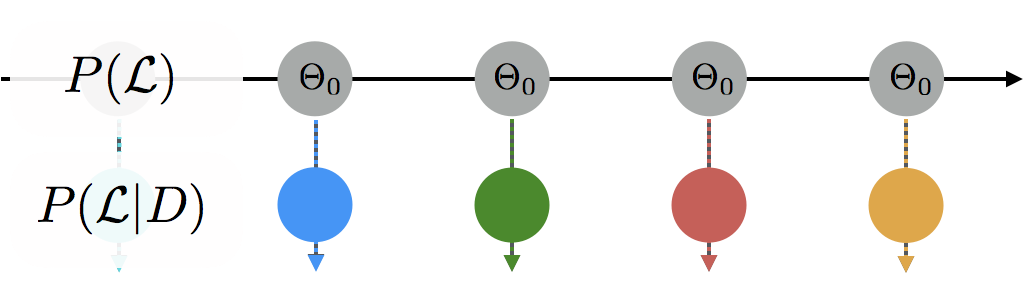
\includegraphics[scale=.4]{model_schematic.png}
\caption{Schematic of our hierarchical model: $\Theta_0$ parameterizes the agent's global beliefs about how their partner uses language, and then through interaction with each partner, they update a partner-specific lexical model based on data $D$ from that interaction.}
\label{fig:modelschematic}
\end{figure}

Now that we have defined a hierarchical likelihood on lexical beliefs, we must say how we \emph{learn} partner-specific models. Our beliefs about a particular partner's lexicon $\mathcal{L}_i$ are formed by integrating our abstract lexical knowledge $\Theta_0$ with particular  observations $D_i$ of that particular individual:
$$%\begin{array}{rcl}
P(\mathcal{L}_i | D_i)  \propto \int_{\Theta_0}P(\mathcal{L}_i | D_i,  \Theta_0) P(\Theta_0 | D_i) 
%                     & = & \mathbb{E}_{\Theta_0}[P(\mathcal{L}_i | \Theta_0, D_i)] 
%\end{array}
$$
where the posteriors in the integral can be computed using Bayes rule:
$$
P(\mathcal{L}_i | D_i, \Theta_0) \propto P(D_i | \mathcal{L}_i, \Theta_0) P(\mathcal{L}_i | \Theta_0)
$$
While this holds when we only have observations from a single speaker, note that our posterior beliefs about $\Theta_0$ are in fact informed by observations from \emph{all} speakers: $D = \bigcup_{i=1}^k D_i$. Finally, to fully specify our model and compute our partner-specific lexical posterior $P(\mathcal{L}_i |D_i, \Theta_0)$, we must link our beliefs about a partner's lexica to their actual behavior with a likelihood function $P(D_i | \mathcal{L}_i, \Theta_0)$. This is naturally supplied by the Rational Speech Act framework: we assume speakers produce utterances that are parsimonious yet informative in context with respect to their lexicon, and listeners interpret utterances by inverting a speaker model. Because we expect our partner to use language rationally given some lexicon, the utterance they choose to refer to some object will be probable under some lexica and highly improbable under others. In this way, a particular agent's language use is a cue to their particular lexicon. 

\begin{figure}[t]
\centering
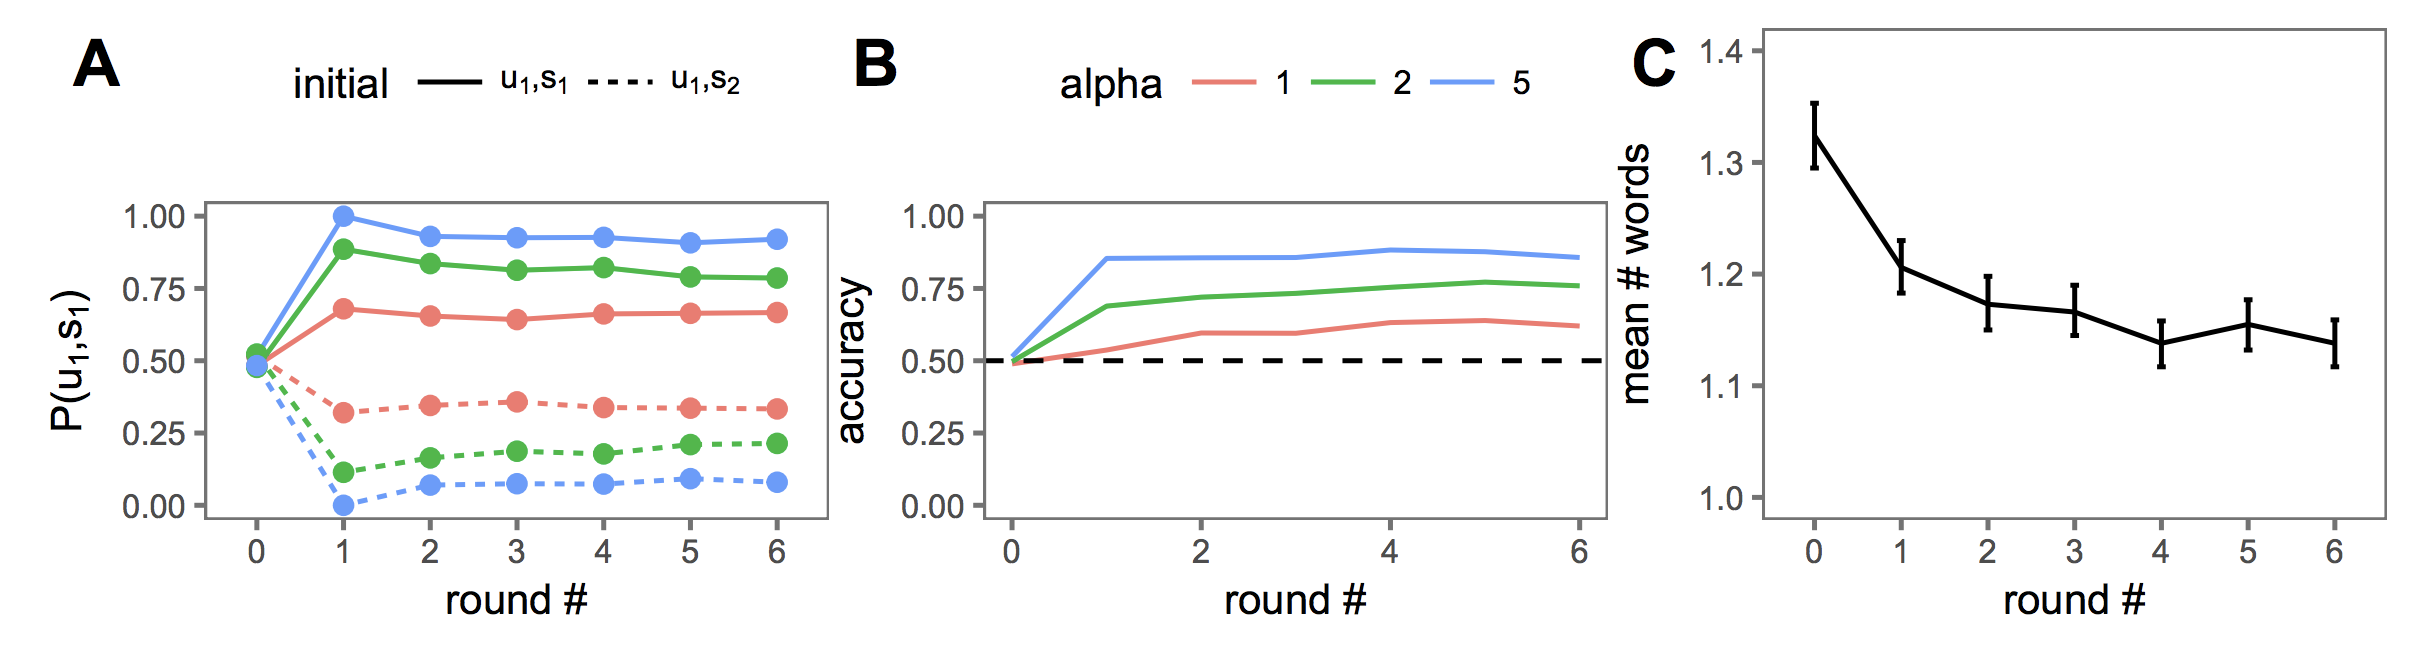
\includegraphics[scale=.36]{model_results.png}
\caption{ (A) Probability of speaker using one of two labels to refer to a state, broken out by initial observation: while players are initially ambivalent between the two labels (arbitrariness), the initial mapping is likely to persist (stability). (B) Accuracy rises as speaker and listener align. (C) When conjunctions are introduced into the grammar, utterances get shorter over time (reduction).}
\label{fig:modelresults}
\end{figure}

First, we show in simulations of a repeated interaction with a single partner that this model successfully allows coordination on arbitrary but path-dependent and stable form-meaning mappings and that a preference for less costly utterances combined with learning gives rise to reduction (see Fig. \ref{fig:modelresults}). Second, we test the generalization properties of our model by manipulating partners and contexts: 
\begin{enumerate}
\item how `sticky' are the pacts formed in one context (i.e. a Dalmatian in the context of other dogs) when the same target is transplanted to a new, less restrictive context (i.e. a Dalmatian in the context of a cat and bear; see Brennen \& Clark, 1996), 
\item to what extent do agents revert to longer utterances after swapping out partners mid-way through a game (see  Wilkes-Gibbs \& Clark, 1992; Metzing \& Brennen, 2003; Yoon \& Brown-Schmidt, 2014), and 
\item how do local, partner-specific expectations generalize to global expectation over repeated interaction with multiple partners in the same community (see Fay et al. 2010).
\end{enumerate}



\section{Chapter 4: How do people coordinate on new conventions in naturalistic interactions?}

A core function of language is \emph{reference}: using words to convey the identity of an object in the environment. 
My research uses a rich, naturalistic communication paradigm called a \emph{repeated reference game} that (1) requires participants to find some way of referring to novel, ambiguous stimuli that they don't already have strong conventions for and (2) asks them to refer to these same objects across multiple rounds as they build up a shared history of interaction, or `common ground,' with their partner.
%In this paradigm, two participants are placed in an interactive environment containing a chat box and an array of objects. 
%On each round of the game, one player---the speaker---is privately shown one object highlighted as the target. 
%The speaker must then produce a message allowing their partner to identify and select the target from their own screen.
%Thus, when participants are pre must coordinate with one another on a way of repeatedly referring to novel, difficult-to-describe tangram shapes. 
I collected a large corpus ($> 15,000$ messages) of the natural language dialogue sent through a chat box by hundreds of pairs of participants playing this game over the web \cite{hawkins_convention-formation_2017}.
I then used recent techniques developed from natural language processing to quantitatively characterize how the structure and content of participants' language evolves as they coordinate on new conventions.

First, going beyond classic work showing that messages get shorter and more efficient across repetitions, I extracted parts of speech and syntax trees from the natural text to understand \emph{what} was reducing and \emph{how}.
I found that pairs systematically drop entire modifying phrases at each repetition, leaving only open-class parts of speech (e.g. an adjective and noun) by the final round. 
Second, I extracted word embeddings (e.g. GloVe vectors) for each message to calculate the similarity of messages within and across pairs. 
I found that while different pairs coordinate on a wide range of idiosyncratic solutions to the problem of reference, they do so in a highly path-dependent manner: words that are more discriminative in the initial context (i.e. that were used for one target more than others) are more likely to persist through the final round.
These findings provide higher resolution into the quantitative dynamics of convention formation: based on usage, existing words systematically acquire new meaning with a partner and support more efficient communication.
%The referring expressions generated by participants across these games reveals a number of rich qualitative phenomena about adaptation in communication. We conduct a large-scale replication of the matching task used by Clark \& Wilkes-Gibbs (1986) as well as a reference game variant with the same stimuli that allows us to track the change in referring expressions over time at a tangram-by-tangram level. We use modern natural language processing techniques to analyze the lexical and syntactic features of utterances and show (1) that the lexical pacts participants form are arbitrary and stable, and (2) that participants are reducing their referring expressions in a systematic and path-dependent manner to preserve distinctive information.

\begin{figure}[t]
\centering
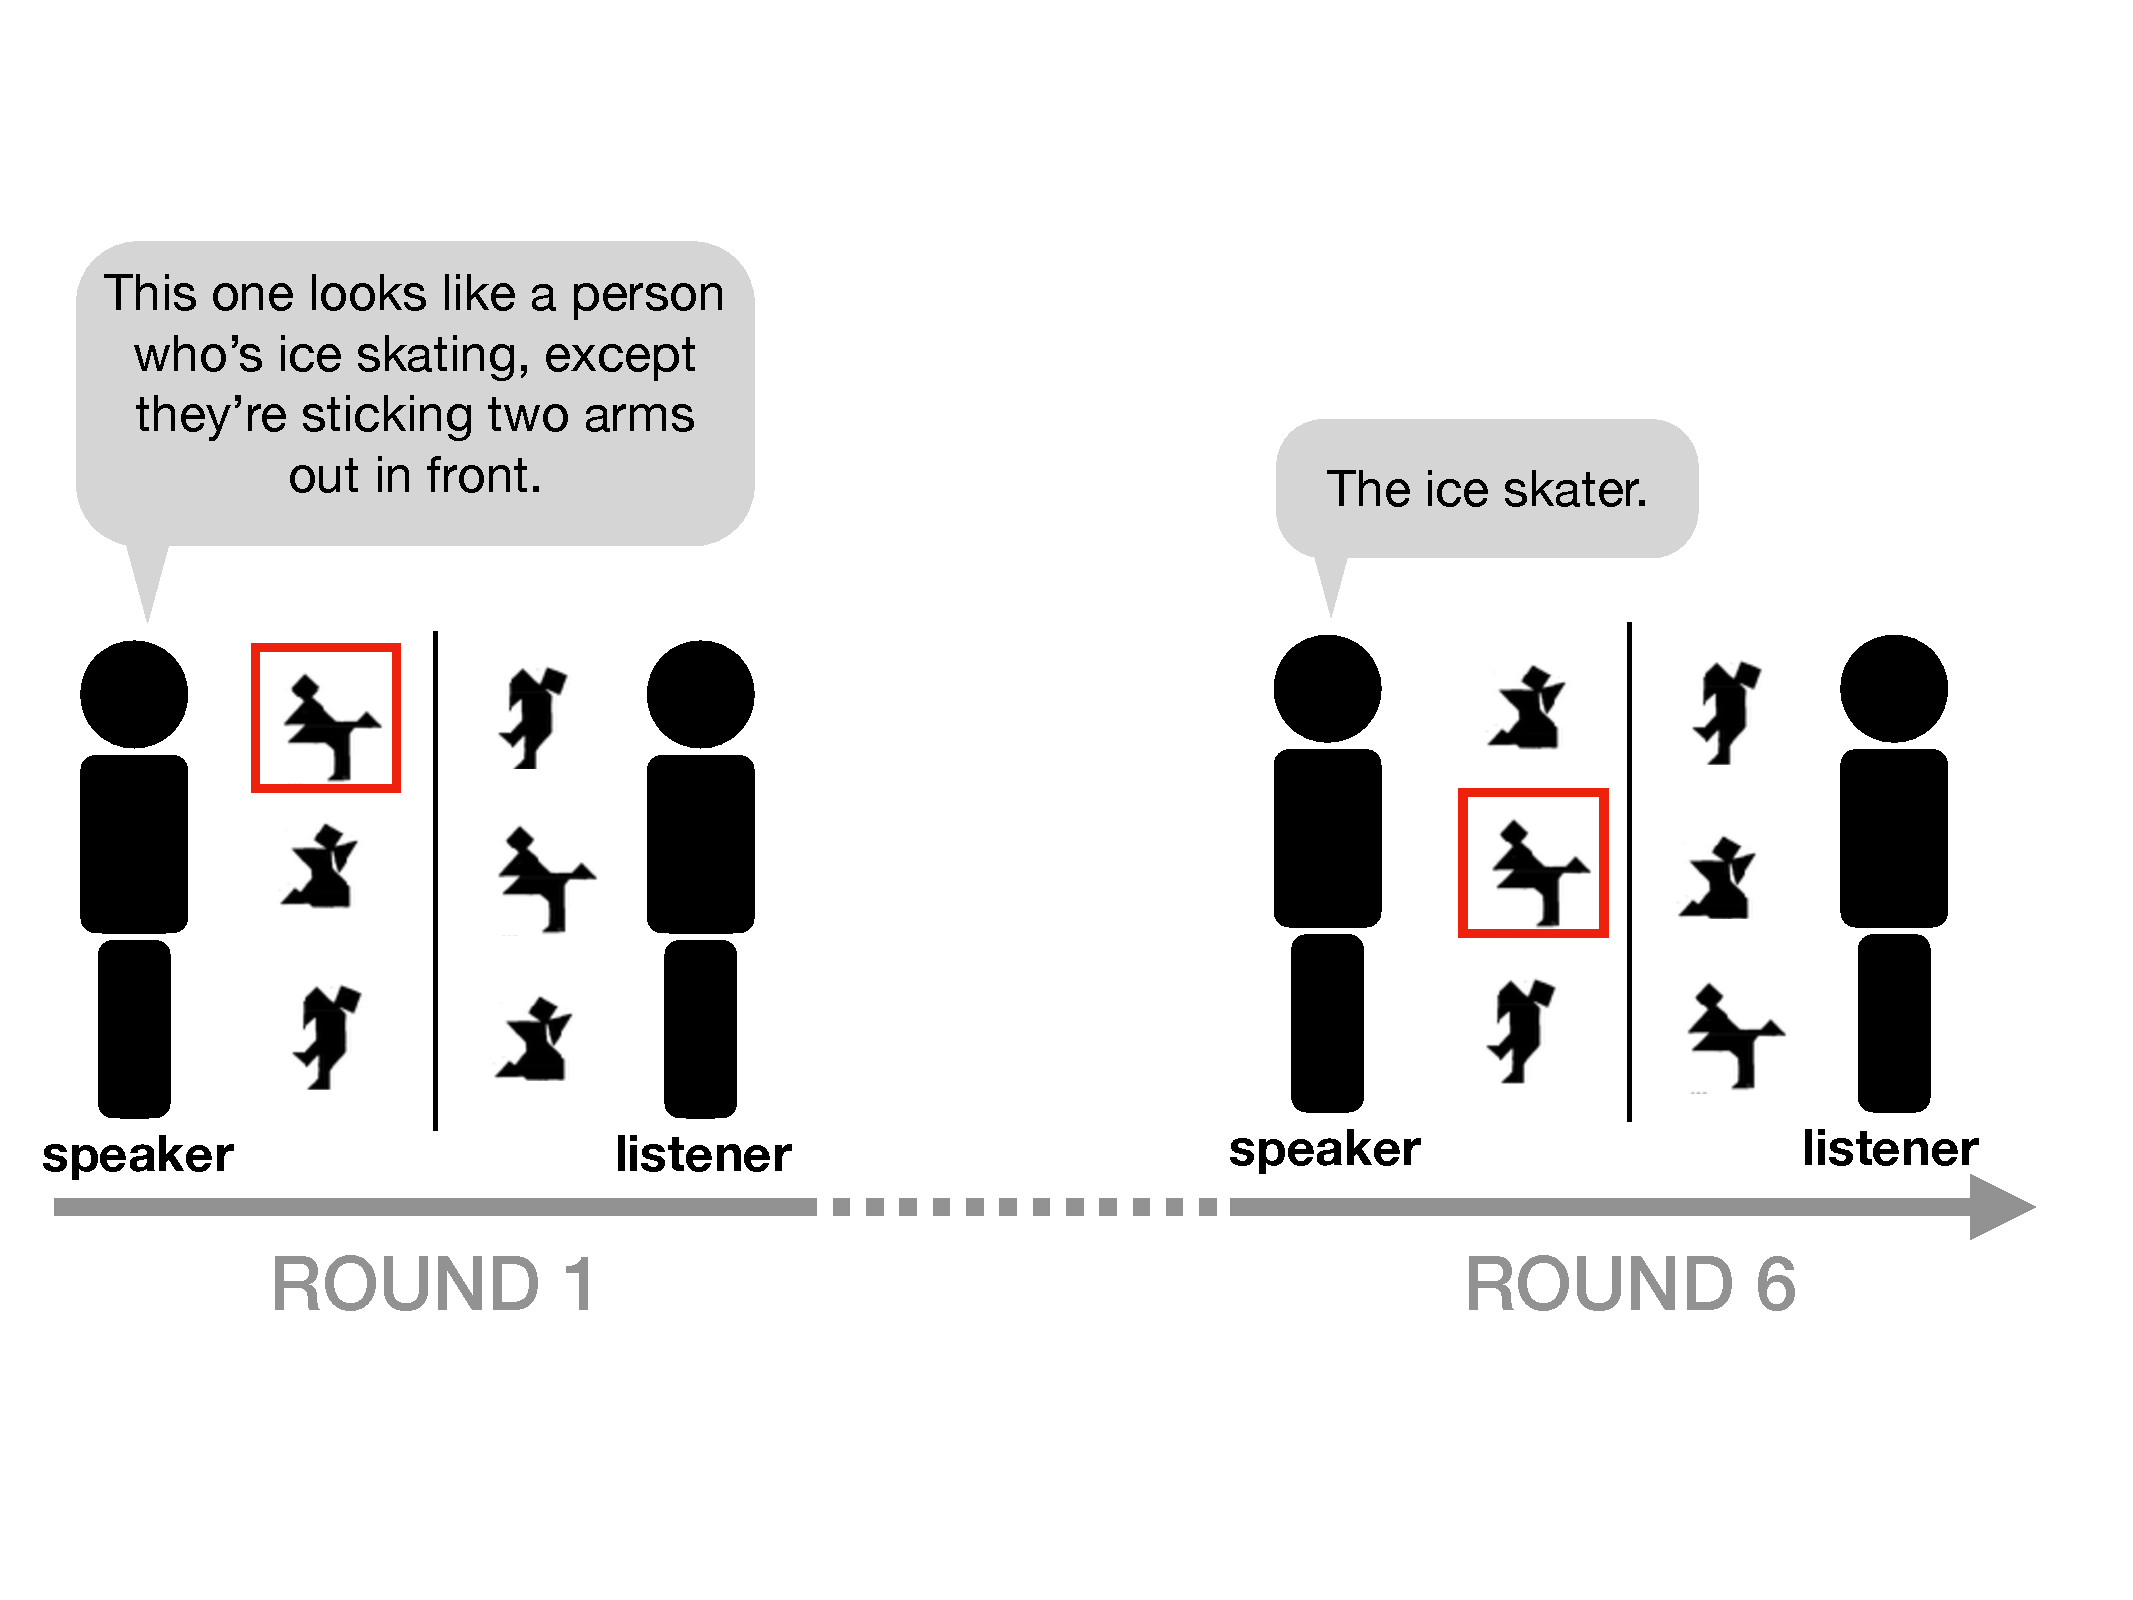
\includegraphics[scale=.45]{task_cropped.pdf}
\caption{Generic setup for repeated reference game task in the lab using stimuli from Wilkes-Gibbs \& Clark (1986); on every round, the speaker refers to each target in some context, and the listener attempts to pick out the intended referent. Both players are free to speak at any time.}
\label{fig:tangramsmethods}
\end{figure}

\begin{figure}[t]
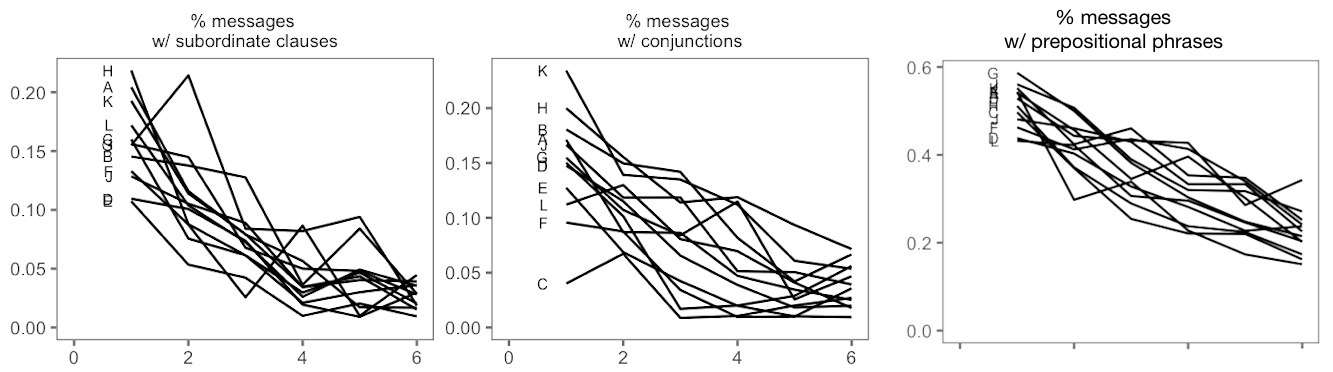
\includegraphics[scale=.35]{tangrams_results.png}
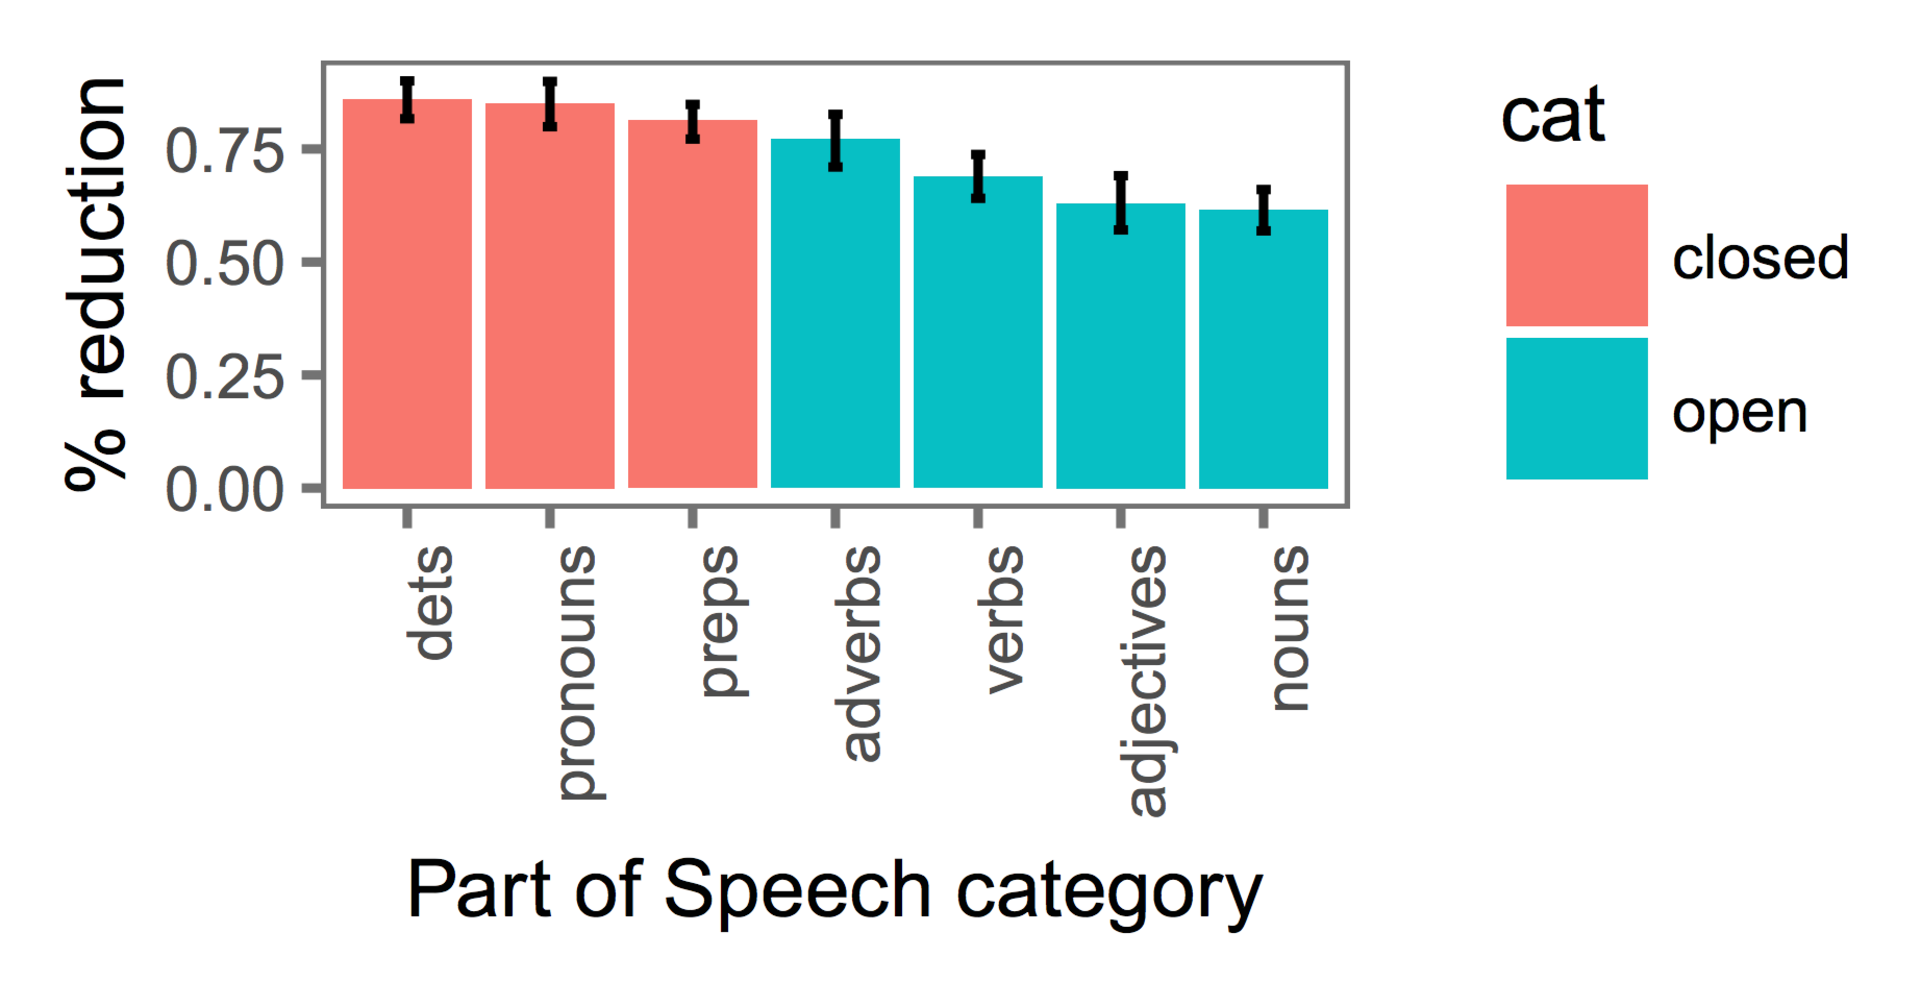
\includegraphics[scale=.25]{pos_fig.pdf}
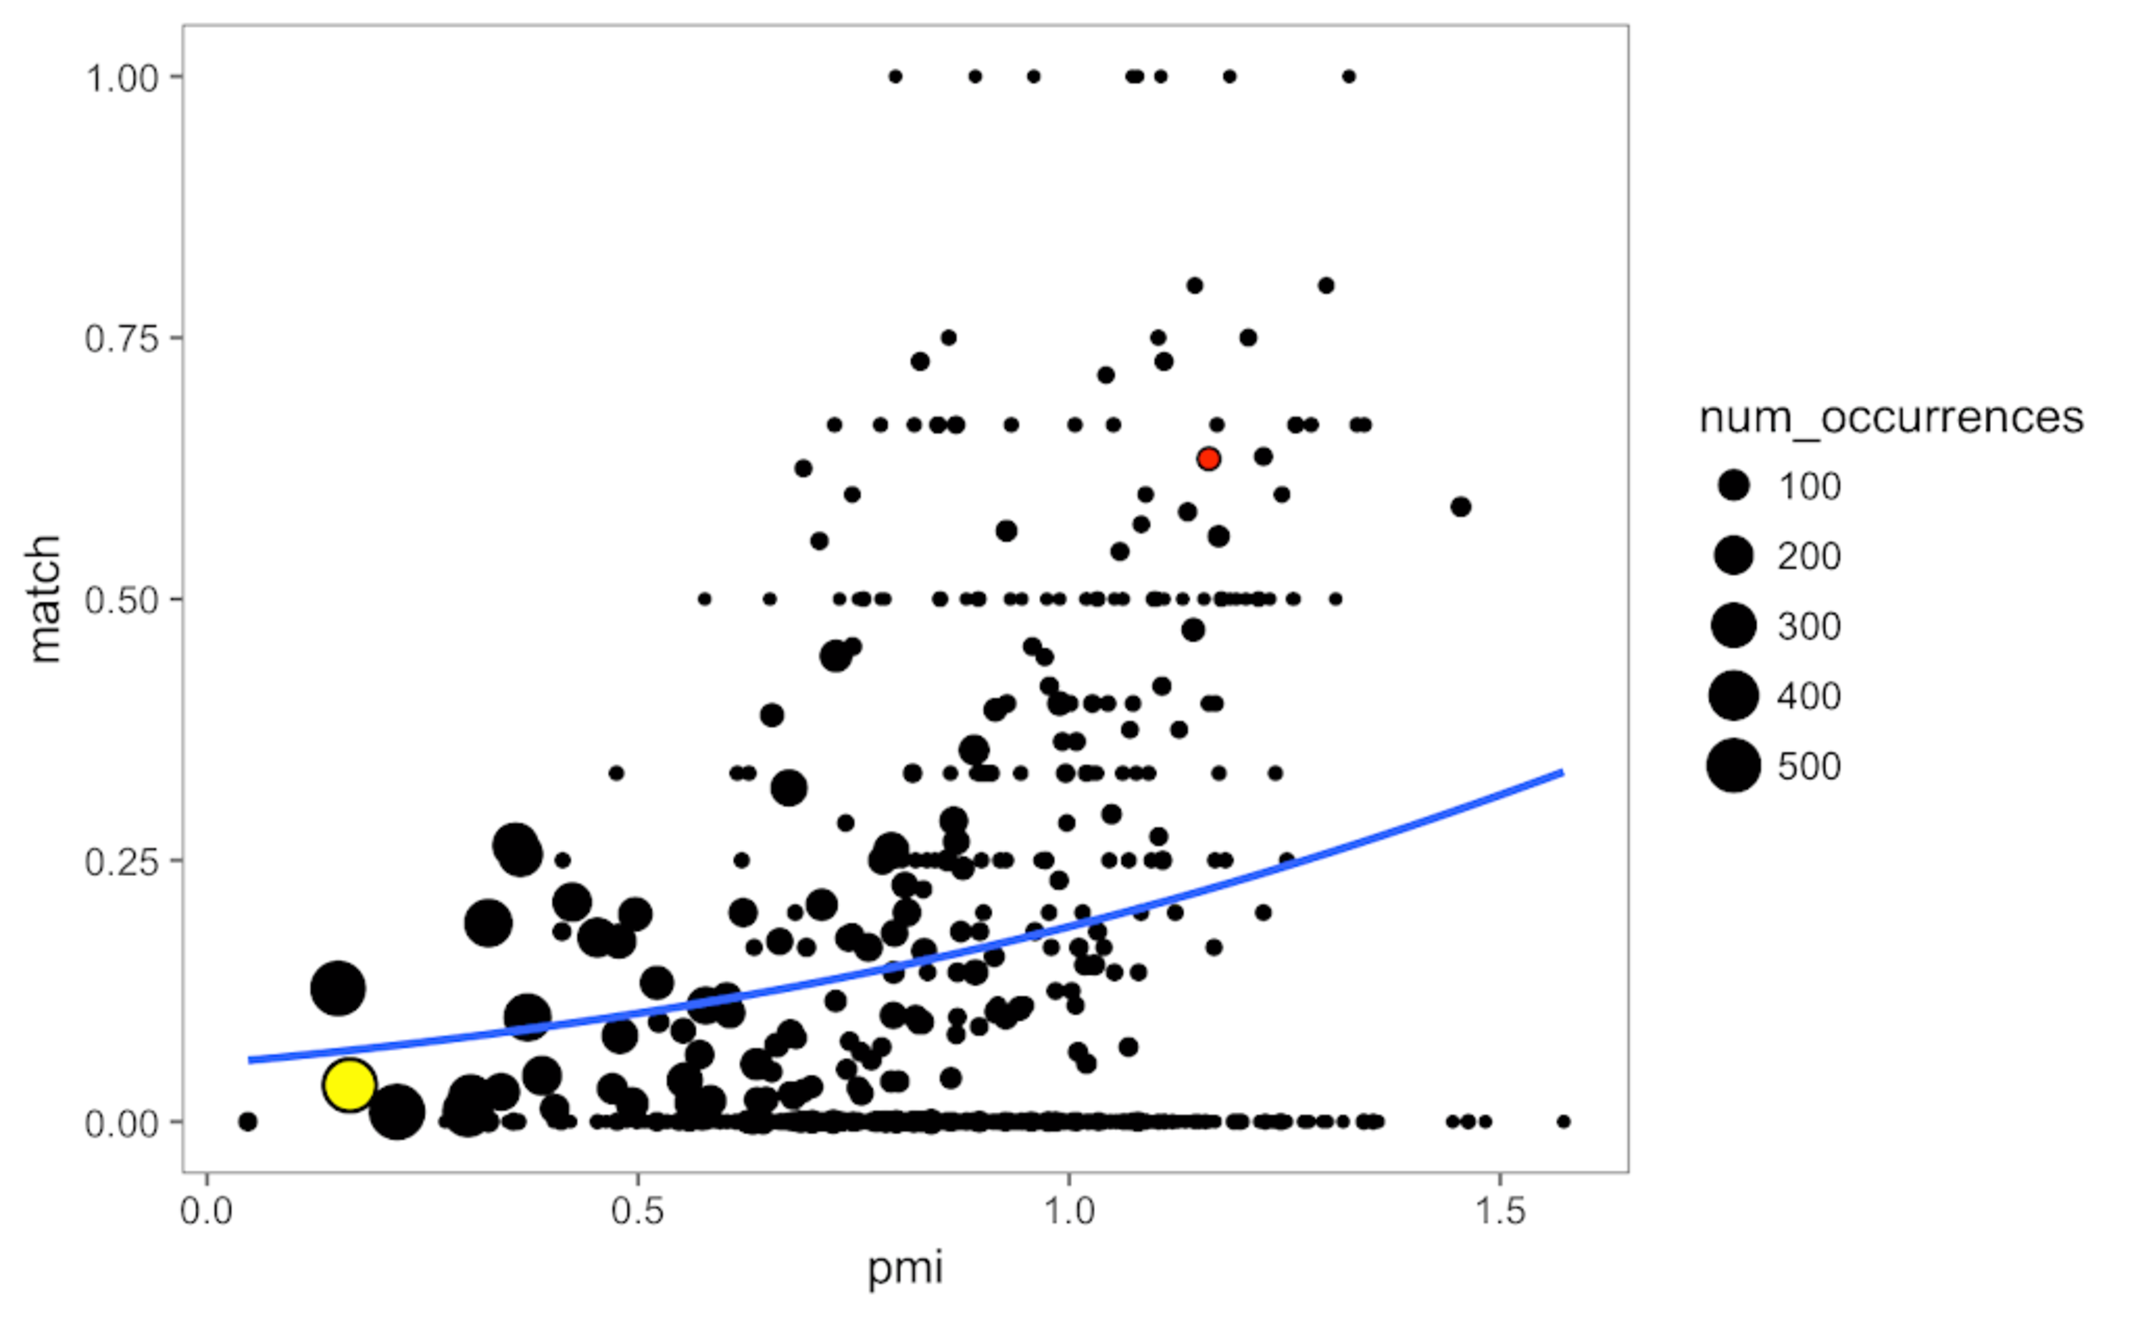
\includegraphics[scale=.25]{pmi.pdf}
\caption{Reduction phenomena reproduced from Hawkins et al, 2017. Clockwise from left: (1) proportion of messages with subordinate clause, broken out by tangram, (2) proportion of messages with conjunction, (3) proportion of utterances containing prepositional phrase, (4) point-wise mutual information on first repetition predicts the likelihood of that word appearing in the final repetition (5) Reduction rates for different parts of speech. Error bars are bootstrapped 95\% CIs}
\label{fig:tangramsresults}
\end{figure}

\vspace{1cm}

\section*{Lexical conventions are shaped by communicative context}

These findings suggest that although there may be many equally effective solutions discovered by different pairs, the resulting conventions are nonetheless \emph{adaptive}: they are shaped by the functional demands of communication in the local environment.
%While this first project emphasized the wide diversity of equally functional labels that different pairs converged on, it also raised new questions about the role of context. 
\textbf{Chapter 5} tests this hypothesis using a controlled artificial-language paradigm adopted from studies of language evolution.
As before, participants were paired to communicate about a set of target objects, but the statistics of the environment were manipulated across different pairs to make different distinctions relevant \cite{hawkins_emerging_abstractions_2018}. 
%This allowed me to remove the stable priors of natural language and isolate the mechanisms of rapid coordination.
In the `fine' condition, distractors were very similar to the target, thus inducing a communicative need for finer distinctions. 
In the `coarse' condition, distractors differed from the target at higher levels of a concept hierarchy.  
%where when the context requires frequently making fine distinctions between entities; conversely, they should converge on a more compressed system of conventions for abstract categories (e.g. dog) in coarser contexts, even if a finer mapping would be sufficient. 
Using a post-test probing the resulting conventions and a statistical approach inferring the lexicon at early stages from usage, I found systematic differences in the \emph{level of abstraction} of conventions in these different contexts. 
%In the coarse condition, participants learned to communicate with smaller vocabularies collapsing over distinctions within categories, while in the fine condition they had more specific labels for sub-categories. 
%Additionally, I introduced a novel statistical approach to probe the dynamics of the lexicon at formative stages by inferring meanings from usage. 
These results indicate that pragmatic considerations of \textit{informativity in context} shape the formation of lexical conventions over longer interactions.

\begin{figure}[b]
\centering
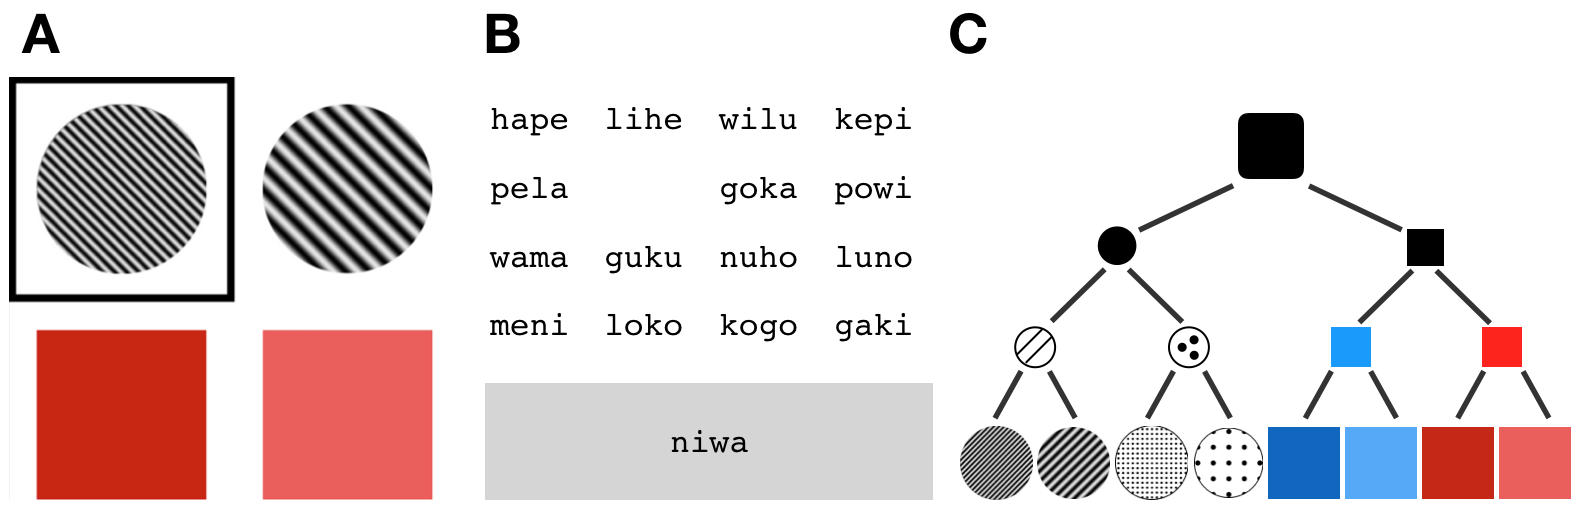
\includegraphics[scale=.5]{fig.png}
\caption{(A) Example of fine context where one of the distractors belongs to the same fine-grained branch of the hierarchy as the target (i.e. another striped circle), so any abstract label would be insufficient to disambiguate them. The target is highlighted for the speaker with a black square. (B) Drag-and-drop chat box interface. (C) Hierarchical organization of stimuli.}
\label{fig:2018task}
\end{figure}

\begin{figure}[t]
\centering
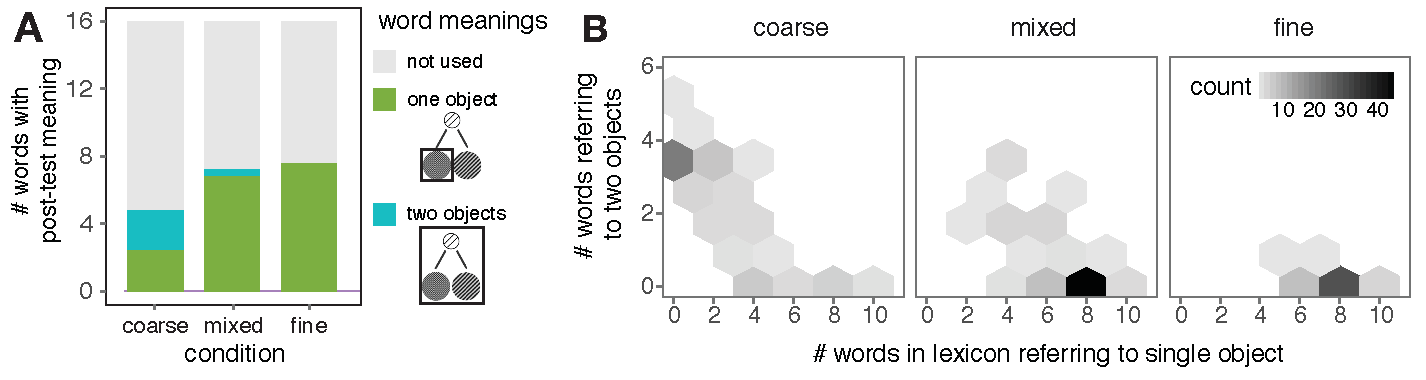
\includegraphics[scale=.7]{resultsFig_v1.pdf}
\caption{ Pragmatic demands of context shape the formation of abstractions. (A) Mean number of words participants reported
with specific meanings (applying to 1 object) or abstract meanings (applying to 2 objects). (B) Diversity of terms within
reported lexica: many participants in the coarse condition reported a mixture of abstract and specific terms.}
\label{fig:modelresults}
\end{figure}

%Words exist for referring at many levels of specificity: from the broadest (thing) to the most specific (Fido). What drives the emergence of these taxonomies of reference? Recent computational theories of language evolution suggest that communicative demands of the environment may play a deciding role. Here, we investigate local pragmatic mechanisms of lexical adaptation that may undergird global emergence by manipulating context in a repeated reference game where pairs of participants interactively coordinate on an artificial communication system (see Fig. \ref{fig:2018task}). We hypothesize that pairs should coordinate on conventions for specific names (e.g. Fido) when the context requires frequently making fine distinctions between entities; conversely, they should converge on a more compressed system of conventions for abstract categories (e.g. dog) in coarser contexts, even if a finer mapping would be sufficient. We show differences in the levels of abstraction that emerged in different environments (see Fig. \ref{fig:2018task}) and introduce a statistical approach to probe the dynamics of emergence. Finally, we use these data as a quantitative test for the model we proposed in Chapter 3. 

%There are \emph{many} potential ways this function could be represented in the mind at the algorithmic level. It could be derived from a store of exemplars, a set of independent prototypes for each word, a neural network embedding words and objects in a vector space, and so on \cite<see>[for a recent review of candidates]{JonesEtAl15_SemanticMemory}.

\section*{Conclusions}


Language is not some monolithic body of knowledge that we acquire at an early age and deploy mechanically for the rest of our lives. Nor is its evolution a slow, inter-generational drift. It is a means for communication -- a shared interface between minds -- and must therefore adapt over the rapid timescales required by communication. In other words, we are constantly learning language. Not just one language, but a large variety of related languages, across every repeated interaction with every partner. 

My research program seeks to understand the core cognitive mechanisms that give rise to human social intelligence.
In pursuit of this goal, I collect rich data from naturalistic social interactions in order to infer sets of candidate mechanisms, and instantiate them in computational cognitive models that reverse-engineer the algorithmic principles of social cognition. 
In addition to making quantitative predictions that address fundamental questions in cognitive science, these models also have broader application potential toward building more socially intelligent AI.
By computationally characterizing these cognitive mechanisms, we will be better positioned to understand how interactions between individuals collectively give rise to human culture. 



%\section{\bf Acknowledgments}
%\small
%\noindent RXDH was supported by the Stanford Graduate Fellowship and the National Science Foundation Graduate Research Fellowship under Grant No. DGE-114747.

\small
\singlespacing
\bibliography{precis}
\bibliographystyle{apacite}


\end{document}  
